% Options for packages loaded elsewhere
\PassOptionsToPackage{unicode}{hyperref}
\PassOptionsToPackage{hyphens}{url}
%
\documentclass[
  ignorenonframetext,
]{beamer}
\usepackage{pgfpages}
\setbeamertemplate{caption}[numbered]
\setbeamertemplate{caption label separator}{: }
\setbeamercolor{caption name}{fg=normal text.fg}
\beamertemplatenavigationsymbolsempty
% Prevent slide breaks in the middle of a paragraph
\widowpenalties 1 10000
\raggedbottom
\setbeamertemplate{part page}{
  \centering
  \begin{beamercolorbox}[sep=16pt,center]{part title}
    \usebeamerfont{part title}\insertpart\par
  \end{beamercolorbox}
}
\setbeamertemplate{section page}{
  \centering
  \begin{beamercolorbox}[sep=12pt,center]{part title}
    \usebeamerfont{section title}\insertsection\par
  \end{beamercolorbox}
}
\setbeamertemplate{subsection page}{
  \centering
  \begin{beamercolorbox}[sep=8pt,center]{part title}
    \usebeamerfont{subsection title}\insertsubsection\par
  \end{beamercolorbox}
}
\AtBeginPart{
  \frame{\partpage}
}
\AtBeginSection{
  \ifbibliography
  \else
    \frame{\sectionpage}
  \fi
}
\AtBeginSubsection{
  \frame{\subsectionpage}
}
\usepackage{amsmath,amssymb}
\usepackage{lmodern}
\usepackage{iftex}
\ifPDFTeX
  \usepackage[T1]{fontenc}
  \usepackage[utf8]{inputenc}
  \usepackage{textcomp} % provide euro and other symbols
\else % if luatex or xetex
  \usepackage{unicode-math}
  \defaultfontfeatures{Scale=MatchLowercase}
  \defaultfontfeatures[\rmfamily]{Ligatures=TeX,Scale=1}
\fi
\usetheme[]{Copenhagen}
\usecolortheme{dolphin}
\usefonttheme{structurebold}
% Use upquote if available, for straight quotes in verbatim environments
\IfFileExists{upquote.sty}{\usepackage{upquote}}{}
\IfFileExists{microtype.sty}{% use microtype if available
  \usepackage[]{microtype}
  \UseMicrotypeSet[protrusion]{basicmath} % disable protrusion for tt fonts
}{}
\makeatletter
\@ifundefined{KOMAClassName}{% if non-KOMA class
  \IfFileExists{parskip.sty}{%
    \usepackage{parskip}
  }{% else
    \setlength{\parindent}{0pt}
    \setlength{\parskip}{6pt plus 2pt minus 1pt}}
}{% if KOMA class
  \KOMAoptions{parskip=half}}
\makeatother
\usepackage{xcolor}
\newif\ifbibliography
\usepackage{color}
\usepackage{fancyvrb}
\newcommand{\VerbBar}{|}
\newcommand{\VERB}{\Verb[commandchars=\\\{\}]}
\DefineVerbatimEnvironment{Highlighting}{Verbatim}{commandchars=\\\{\}}
% Add ',fontsize=\small' for more characters per line
\usepackage{framed}
\definecolor{shadecolor}{RGB}{248,248,248}
\newenvironment{Shaded}{\begin{snugshade}}{\end{snugshade}}
\newcommand{\AlertTok}[1]{\textcolor[rgb]{0.94,0.16,0.16}{#1}}
\newcommand{\AnnotationTok}[1]{\textcolor[rgb]{0.56,0.35,0.01}{\textbf{\textit{#1}}}}
\newcommand{\AttributeTok}[1]{\textcolor[rgb]{0.77,0.63,0.00}{#1}}
\newcommand{\BaseNTok}[1]{\textcolor[rgb]{0.00,0.00,0.81}{#1}}
\newcommand{\BuiltInTok}[1]{#1}
\newcommand{\CharTok}[1]{\textcolor[rgb]{0.31,0.60,0.02}{#1}}
\newcommand{\CommentTok}[1]{\textcolor[rgb]{0.56,0.35,0.01}{\textit{#1}}}
\newcommand{\CommentVarTok}[1]{\textcolor[rgb]{0.56,0.35,0.01}{\textbf{\textit{#1}}}}
\newcommand{\ConstantTok}[1]{\textcolor[rgb]{0.00,0.00,0.00}{#1}}
\newcommand{\ControlFlowTok}[1]{\textcolor[rgb]{0.13,0.29,0.53}{\textbf{#1}}}
\newcommand{\DataTypeTok}[1]{\textcolor[rgb]{0.13,0.29,0.53}{#1}}
\newcommand{\DecValTok}[1]{\textcolor[rgb]{0.00,0.00,0.81}{#1}}
\newcommand{\DocumentationTok}[1]{\textcolor[rgb]{0.56,0.35,0.01}{\textbf{\textit{#1}}}}
\newcommand{\ErrorTok}[1]{\textcolor[rgb]{0.64,0.00,0.00}{\textbf{#1}}}
\newcommand{\ExtensionTok}[1]{#1}
\newcommand{\FloatTok}[1]{\textcolor[rgb]{0.00,0.00,0.81}{#1}}
\newcommand{\FunctionTok}[1]{\textcolor[rgb]{0.00,0.00,0.00}{#1}}
\newcommand{\ImportTok}[1]{#1}
\newcommand{\InformationTok}[1]{\textcolor[rgb]{0.56,0.35,0.01}{\textbf{\textit{#1}}}}
\newcommand{\KeywordTok}[1]{\textcolor[rgb]{0.13,0.29,0.53}{\textbf{#1}}}
\newcommand{\NormalTok}[1]{#1}
\newcommand{\OperatorTok}[1]{\textcolor[rgb]{0.81,0.36,0.00}{\textbf{#1}}}
\newcommand{\OtherTok}[1]{\textcolor[rgb]{0.56,0.35,0.01}{#1}}
\newcommand{\PreprocessorTok}[1]{\textcolor[rgb]{0.56,0.35,0.01}{\textit{#1}}}
\newcommand{\RegionMarkerTok}[1]{#1}
\newcommand{\SpecialCharTok}[1]{\textcolor[rgb]{0.00,0.00,0.00}{#1}}
\newcommand{\SpecialStringTok}[1]{\textcolor[rgb]{0.31,0.60,0.02}{#1}}
\newcommand{\StringTok}[1]{\textcolor[rgb]{0.31,0.60,0.02}{#1}}
\newcommand{\VariableTok}[1]{\textcolor[rgb]{0.00,0.00,0.00}{#1}}
\newcommand{\VerbatimStringTok}[1]{\textcolor[rgb]{0.31,0.60,0.02}{#1}}
\newcommand{\WarningTok}[1]{\textcolor[rgb]{0.56,0.35,0.01}{\textbf{\textit{#1}}}}
\setlength{\emergencystretch}{3em} % prevent overfull lines
\providecommand{\tightlist}{%
  \setlength{\itemsep}{0pt}\setlength{\parskip}{0pt}}
\setcounter{secnumdepth}{-\maxdimen} % remove section numbering
\ifLuaTeX
  \usepackage{selnolig}  % disable illegal ligatures
\fi
\IfFileExists{bookmark.sty}{\usepackage{bookmark}}{\usepackage{hyperref}}
\IfFileExists{xurl.sty}{\usepackage{xurl}}{} % add URL line breaks if available
\urlstyle{same} % disable monospaced font for URLs
\hypersetup{
  pdfauthor={Alex Sanchez, Miriam Mota, Ricardo Gonzalo and Santi Pérez},
  hidelinks,
  pdfcreator={LaTeX via pandoc}}

\title{Statistical Analysis with R: Data Management and Automation}
\author{Alex Sanchez, Miriam Mota, Ricardo Gonzalo and Santi Pérez}
\date{Statistics and Bioinformatics Unit. Vall d'Hebron Institut de
Recerca}

\begin{document}
\frame{\titlepage}

\begin{frame}{Outline: Data Exploration*}
\protect\hypertarget{outline-data-exploration}{}
\vspace{2cm}

\begin{itemize}
\tightlist
\item
  Data managements with dplyr
\item
  The pipe operator \%\textgreater\%
\item
  Merging datasets
\end{itemize}

\vspace{2.5cm}

\tiny *Based on this presentation:
\href{https://stats.idre.ucla.edu/stat/data/rdm/data_management_seminar.html\#153}{\emph{Data
Managment, UCLA}}.
\end{frame}

\begin{frame}[fragile]{Data Management packages}
\protect\hypertarget{data-management-packages}{}
\textbf{tidyverse:} a collection of packages with tools for most aspects
of data analysis, particularly strong in data import, management, and
visualization. Packages within tidyverse:

\begin{itemize}
\tightlist
\item
  \textbf{dplyr} - subsetting, sorting, transforming variables, grouping
\item
  \textbf{tidyr} - restructuring rows and columns
\item
  \textbf{magrittr} - piping a chain of commands
\item
  \textbf{stringr} - string variable manipulation
\end{itemize}

\footnotesize

\begin{Shaded}
\begin{Highlighting}[]
\CommentTok{\# install.packages("tidyverse", dependencies = TRUE)}
\FunctionTok{library}\NormalTok{(tidyverse)}
\end{Highlighting}
\end{Shaded}

\normalsize
\end{frame}

\begin{frame}{Example dataset}
\protect\hypertarget{example-dataset}{}
\begin{figure}
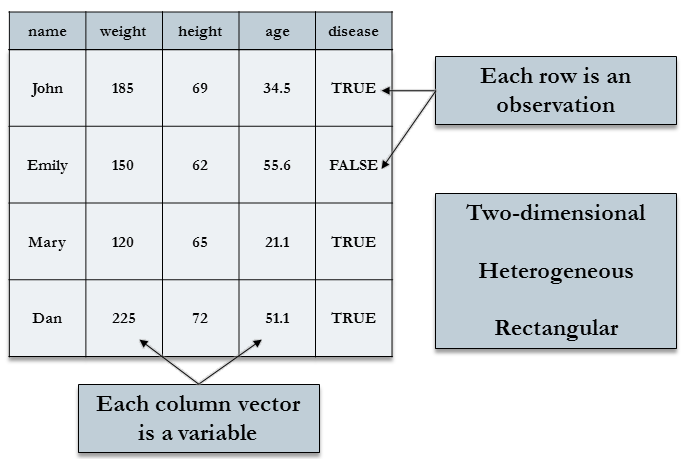
\includegraphics[width=.9\linewidth]{images/dataset.png}
\end{figure}
\end{frame}

\hypertarget{data-managements-with-dplyr}{%
\section{Data managements with
dplyr}\label{data-managements-with-dplyr}}

\begin{frame}{The dplyr package}
\protect\hypertarget{the-dplyr-package}{}
The \textbf{dplyr} package provides tools for some of the most common
data management tasks. Its primary functions are ``verbs'' to help you
think about what you need to do to your dataset:

\begin{itemize}
\tightlist
\item
  \textbf{filter()}: select rows according to conditions
\item
  \textbf{select()}: select columns (you can rename as you select)
\item
  \textbf{arrange()}: sort rows
\item
  \textbf{mutate()}: add new columns
\end{itemize}

The \textbf{dplyr} package is automatically loaded with
\textbf{library(tidyverse)}.
\end{frame}

\begin{frame}[fragile]{Selecting rows with filter}
\protect\hypertarget{selecting-rows-with-filter}{}
The dplyr function filter() provides a cleaner syntax for subsetting
datasets. Conditions separated by , are joined by \& (logical AND).

\footnotesize

\begin{Shaded}
\begin{Highlighting}[]
\FunctionTok{require}\NormalTok{(readxl)}
\NormalTok{diab }\OtherTok{\textless{}{-}} \FunctionTok{read\_excel}\NormalTok{(}\StringTok{"datasets/diabetes.xls"}\NormalTok{)}
\NormalTok{diab\_filt }\OtherTok{\textless{}{-}} \FunctionTok{filter}\NormalTok{(diab, tabac }\SpecialCharTok{==} \StringTok{"No fumador"}\NormalTok{, edat }\SpecialCharTok{\textgreater{}=} \DecValTok{50}\NormalTok{)}
\FunctionTok{head}\NormalTok{(diab\_filt, }\AttributeTok{n =} \DecValTok{4}\NormalTok{)}
\end{Highlighting}
\end{Shaded}

\begin{verbatim}
## # A tibble: 4 x 11
##   numpacie mort   tempsviu  edat   bmi edatdiag tabac      sbp   dbp ecg   chd  
##      <dbl> <chr>     <dbl> <dbl> <dbl>    <dbl> <chr>    <dbl> <dbl> <chr> <chr>
## 1        7 Vivo       12.4    50  36.5       48 No fuma~   140    86 Fron~ Si   
## 2       12 Vivo       10.8    54  42.9       43 No fuma~   128    74 Norm~ No   
## 3       56 Vivo       10.2    64  30.1       58 No fuma~   138    76 Fron~ Si   
## 4       59 Muerto      6.7    62  34.6       58 No fuma~   138    78 Anor~ Si
\end{verbatim}

\normalsize
\end{frame}

\begin{frame}[fragile]{Selecting columns with select}
\protect\hypertarget{selecting-columns-with-select}{}
Use dplyr function select() to keep only the variables you need.

\footnotesize

\begin{Shaded}
\begin{Highlighting}[]
\NormalTok{diab\_small }\OtherTok{\textless{}{-}} \FunctionTok{select}\NormalTok{(diab, mort, edat, tabac, sbp)}
\FunctionTok{head}\NormalTok{(diab\_small, }\AttributeTok{n =} \DecValTok{4}\NormalTok{)}
\end{Highlighting}
\end{Shaded}

\begin{verbatim}
## # A tibble: 4 x 4
##   mort   edat tabac        sbp
##   <chr> <dbl> <chr>      <dbl>
## 1 Vivo     44 No fumador   132
## 2 Vivo     49 Fumador      130
## 3 Vivo     49 Fumador      108
## 4 Vivo     47 No fumador   128
\end{verbatim}

\normalsize
\end{frame}

\begin{frame}[fragile]{Sorting rows with arrange}
\protect\hypertarget{sorting-rows-with-arrange}{}
Sort the order of rows by variable values using \textbf{arrange()} from
dplyr.

Be default, ascending order will be used. Surround a sorting variable
with \textbf{desc()} to sort by descending order instead.

\footnotesize

\begin{Shaded}
\begin{Highlighting}[]
\CommentTok{\# sort, with males before \textquotesingle{}vivo\textquotesingle{}, then by age, youngest first}
\NormalTok{diab\_sort }\OtherTok{\textless{}{-}} \FunctionTok{arrange}\NormalTok{(diab, }\FunctionTok{desc}\NormalTok{(mort), edat) }
\FunctionTok{head}\NormalTok{(diab\_sort, }\AttributeTok{n =} \DecValTok{4}\NormalTok{)}
\end{Highlighting}
\end{Shaded}

\begin{verbatim}
## # A tibble: 4 x 11
##   numpacie mort  tempsviu  edat   bmi edatdiag tabac       sbp   dbp ecg   chd  
##      <dbl> <chr>    <dbl> <dbl> <dbl>    <dbl> <chr>     <dbl> <dbl> <chr> <chr>
## 1      114 Vivo      14.8    31  38.8       29 Ex fumad~   136    76 Norm~ No   
## 2      110 Vivo      15.4    33  34         33 Fumador     120    78 Norm~ No   
## 3       27 Vivo       8.6    34  33.9       30 Fumador     124    66 Norm~ No   
## 4       20 Vivo      14.1    35  47         33 Ex fumad~   134    78 Norm~ No
\end{verbatim}

\normalsize
\end{frame}

\begin{frame}{R Logical operators and functions}
\protect\hypertarget{r-logical-operators-and-functions}{}
Here are some operators and functions to help with selection:

\begin{itemize}
\tightlist
\item
  \textbf{==}: equality
\item
  \textbf{\(>, >=\)}: greater than, greater than or equal to
\item
  \textbf{!}: not
\item
  \textbf{\&}: AND
\item
  \textbf{\textbar{}}: OR
\item
  \textbf{\%in\%}: matches any of (2 \%in\% c(1,2,3) = TRUE)
\item
  \textbf{is.na()}: equality to NA
\item
  \textbf{near()}: checking for equality for floating point (decimal)
  numbers, has a built-in tolerance
\end{itemize}
\end{frame}

\begin{frame}{Transforming variables into new variables}
\protect\hypertarget{transforming-variables-into-new-variables}{}
The function \textbf{mutate()} allows us to transform many variables in
one step without having to respecify the data frame name over and over.

Useful R functions for transforming:

\begin{itemize}
\tightlist
\item
  \textbf{log()}: logarithm
\item
  \textbf{min\_rank()}: rank values
\item
  \textbf{cut()}: cut a continuous variable into intervals with new
  integer value signifying into which interval original value falls
\item
  \textbf{scale()}: standardizes variable (substracts mean and divides
  by standard deviation)
\item
  \textbf{cumsum()}: cumulative sum
\item
  \textbf{rowMeans(), rowSums()}: means and sums of several columns
\end{itemize}
\end{frame}

\begin{frame}[fragile]{Example: mutate()}
\protect\hypertarget{example-mutate}{}
create age category variable, and highbmi binary variable \tiny

\begin{Shaded}
\begin{Highlighting}[]
\NormalTok{diab\_mut }\OtherTok{\textless{}{-}} \FunctionTok{mutate}\NormalTok{(diab,}
            \AttributeTok{edatcat =} \FunctionTok{cut}\NormalTok{(edat, }\AttributeTok{breaks =} \FunctionTok{c}\NormalTok{(}\DecValTok{0}\NormalTok{,}\DecValTok{40}\NormalTok{,}\DecValTok{50}\NormalTok{,}\DecValTok{60}\NormalTok{,}\DecValTok{70}\NormalTok{,}\DecValTok{120}\NormalTok{)),}
            \AttributeTok{highbmi =}\NormalTok{ bmi }\SpecialCharTok{\textgreater{}} \FunctionTok{mean}\NormalTok{(bmi))}
\FunctionTok{tail}\NormalTok{(diab\_mut, }\AttributeTok{n =} \DecValTok{4}\NormalTok{)}
\end{Highlighting}
\end{Shaded}

\begin{verbatim}
## # A tibble: 4 x 13
##   numpacie mort   tempsviu  edat   bmi edatdiag tabac      sbp   dbp ecg   chd  
##      <dbl> <chr>     <dbl> <dbl> <dbl>    <dbl> <chr>    <dbl> <dbl> <chr> <chr>
## 1      146 Vivo       11      40  34         38 Fumador    132    76 Norm~ No   
## 2      147 Vivo        7.3    61  19.9       37 No fuma~   120    60 Fron~ Si   
## 3      148 Muerto     10.6    62  30.6       49 No fuma~   160    86 Fron~ Si   
## 4      149 Vivo       10.5    49  30.8       47 Ex fuma~   146    86 Norm~ No   
## # ... with 2 more variables: edatcat <fct>, highbmi <lgl>
\end{verbatim}

\normalsize

\footnotesize

\begin{Shaded}
\begin{Highlighting}[]
\FunctionTok{table}\NormalTok{(diab\_mut}\SpecialCharTok{$}\NormalTok{edatcat, diab\_mut}\SpecialCharTok{$}\NormalTok{highbmi)}
\end{Highlighting}
\end{Shaded}

\normalsize
\end{frame}

\begin{frame}{EXERCISE}
\protect\hypertarget{exercise}{}
\begin{enumerate}
\item
  Find all individual that:

  1.1 Had a sbp higher than 160 (\textbf{filter()})

  1.2 Had a sbp higher than 160 or tabac was `Fumador'
\item
  What happens if you include the name of a variable multiple times in a
  \textbf{select()} call?
\item
  Sort individual to find the most `tempsviu'. (\textbf{arrange() })
\end{enumerate}

\footnotesize

\normalsize
\end{frame}

\hypertarget{the-pipe-operator}{%
\section{The pipe operator \%\textgreater\%}\label{the-pipe-operator}}

\begin{frame}{The pipe operator \%\textgreater\%}
\protect\hypertarget{the-pipe-operator-1}{}
A data management task may involve many steps to reach the final desired
dataset. Often, during intermediate steps, datasets are generated that
we don't care about or plan on keeping. For these multi-step tasks, the
pipe operator provides a useful, time-saving and code-saving shorthand.

Naming datasets takes time to think about and clutters code. Piping
makes your code more readable by focusing on the functions used rather
than the name of datasets.
\end{frame}

\begin{frame}{Using the pipe operator}
\protect\hypertarget{using-the-pipe-operator}{}
The pipe operator ``pipes'' the dataset on the left of the
\%\textgreater\% operator to the function on the right of the operator.

The code x \%\textgreater\% f(y) translates to f(x,y), that is, x is
treated by default as the first argument of f(). If the function returns
a data frame, we can then pipe this data frame into another function.
Thus x \%\textgreater\% f(y) \%\textgreater\% g(z) translates to
g(f(x,y), z).
\end{frame}

\begin{frame}[fragile]{Examples of using the pipe operator}
\protect\hypertarget{examples-of-using-the-pipe-operator}{}
As a first example, perhaps we want to create a dataset of just Vivo
under 40, with only the age and pain variables selected. We could do
this in 2 steps, like so:

\footnotesize

\begin{Shaded}
\begin{Highlighting}[]
\NormalTok{diab40 }\OtherTok{\textless{}{-}} \FunctionTok{filter}\NormalTok{(diab, mort }\SpecialCharTok{==} \StringTok{"Vivo"} \SpecialCharTok{\&}\NormalTok{ edat }\SpecialCharTok{\textless{}} \DecValTok{40}\NormalTok{)}
\NormalTok{diab40\_small }\OtherTok{\textless{}{-}} \FunctionTok{select}\NormalTok{(diab40, edat, dbp)}
\FunctionTok{head}\NormalTok{(diab40\_small,}\AttributeTok{n =} \DecValTok{4}\NormalTok{)}
\end{Highlighting}
\end{Shaded}

\begin{verbatim}
## # A tibble: 4 x 2
##    edat   dbp
##   <dbl> <dbl>
## 1    36    88
## 2    38    98
## 3    35    78
## 4    34    66
\end{verbatim}

\normalsize
\end{frame}

\begin{frame}[fragile]{Examples of using the pipe operator}
\protect\hypertarget{examples-of-using-the-pipe-operator-1}{}
While that works fine, the intermediate dataset f40 is not of interest
and is cluttering up memory and the workspace unnecessarily.

We could use \%\textgreater\% instead:

\footnotesize

\begin{Shaded}
\begin{Highlighting}[]
\NormalTok{diab40\_small }\OtherTok{\textless{}{-}}\NormalTok{ diab }\SpecialCharTok{\%\textgreater{}\%}   
  \FunctionTok{filter}\NormalTok{(mort }\SpecialCharTok{==} \StringTok{"Vivo"} \SpecialCharTok{\&}\NormalTok{ edat }\SpecialCharTok{\textless{}} \DecValTok{40}\NormalTok{) }\SpecialCharTok{\%\textgreater{}\%} 
  \FunctionTok{select}\NormalTok{(edat, dbp)}
\FunctionTok{head}\NormalTok{(diab40\_small,}\AttributeTok{n =} \DecValTok{4}\NormalTok{)}
\end{Highlighting}
\end{Shaded}

\begin{verbatim}
## # A tibble: 4 x 2
##    edat   dbp
##   <dbl> <dbl>
## 1    36    88
## 2    38    98
## 3    35    78
## 4    34    66
\end{verbatim}

\normalsize
\end{frame}

\begin{frame}[fragile]{EXERCISE}
\protect\hypertarget{exercise-1}{}
Replicate the last exercice using `pipes'

\footnotesize

\begin{Shaded}
\begin{Highlighting}[]
\NormalTok{df }\OtherTok{\textless{}{-}} \FunctionTok{filter}\NormalTok{(diab,sbp }\SpecialCharTok{\textgreater{}} \DecValTok{160} \SpecialCharTok{|}\NormalTok{ tabac }\SpecialCharTok{==} \StringTok{"Fumador"}\NormalTok{)}

\NormalTok{dfs }\OtherTok{\textless{}{-}} \FunctionTok{select}\NormalTok{(df, tempsviu ,bmi,sbp,sbp)}

\NormalTok{dfsa }\OtherTok{\textless{}{-}} \FunctionTok{arrange}\NormalTok{(dfs, }\FunctionTok{desc}\NormalTok{(tempsviu))}
\end{Highlighting}
\end{Shaded}

\normalsize

\footnotesize

\normalsize
\end{frame}

\hypertarget{merging-datasets}{%
\section{Merging datasets}\label{merging-datasets}}

\begin{frame}{Merging datasets}
\protect\hypertarget{merging-datasets-1}{}
Appending adds more rows of observations, whereas merging adds more
columns of variables. Datasets to be merged should be matched on some id
variable(s).

\begin{figure}
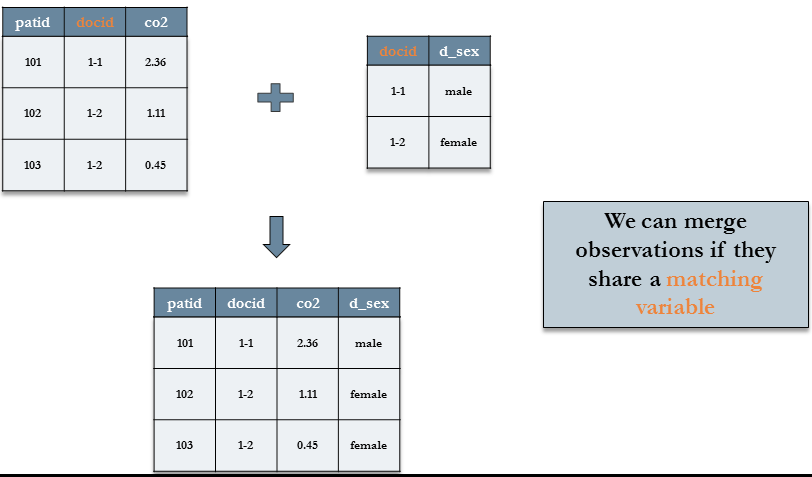
\includegraphics[width=.83\linewidth]{images/merge.png}
\end{figure}
\end{frame}

\begin{frame}[fragile]{Data example}
\protect\hypertarget{data-example}{}
\footnotesize

\begin{Shaded}
\begin{Highlighting}[]
\NormalTok{band\_members}
\end{Highlighting}
\end{Shaded}

\begin{verbatim}
## # A tibble: 3 x 2
##   name  band   
##   <chr> <chr>  
## 1 Mick  Stones 
## 2 John  Beatles
## 3 Paul  Beatles
\end{verbatim}

\begin{Shaded}
\begin{Highlighting}[]
\NormalTok{band\_instruments}
\end{Highlighting}
\end{Shaded}

\begin{verbatim}
## # A tibble: 3 x 2
##   name  plays 
##   <chr> <chr> 
## 1 John  guitar
## 2 Paul  bass  
## 3 Keith guitar
\end{verbatim}

\normalsize
\end{frame}

\begin{frame}[fragile]{Append row bind\_rows()}
\protect\hypertarget{append-row-bind_rows}{}
\footnotesize

\begin{Shaded}
\begin{Highlighting}[]
\FunctionTok{bind\_rows}\NormalTok{(band\_members, band\_instruments)}
\end{Highlighting}
\end{Shaded}

\begin{verbatim}
## # A tibble: 6 x 3
##   name  band    plays 
##   <chr> <chr>   <chr> 
## 1 Mick  Stones  <NA>  
## 2 John  Beatles <NA>  
## 3 Paul  Beatles <NA>  
## 4 John  <NA>    guitar
## 5 Paul  <NA>    bass  
## 6 Keith <NA>    guitar
\end{verbatim}

\normalsize
\end{frame}

\begin{frame}[fragile]{Append columns bind\_cols()}
\protect\hypertarget{append-columns-bind_cols}{}
!!!!!!!!!!

\footnotesize

\begin{Shaded}
\begin{Highlighting}[]
\FunctionTok{bind\_cols}\NormalTok{(band\_members, band\_instruments)}
\end{Highlighting}
\end{Shaded}

\begin{verbatim}
## New names:
## * `name` -> `name...1`
## * `name` -> `name...3`
\end{verbatim}

\begin{verbatim}
## # A tibble: 3 x 4
##   name...1 band    name...3 plays 
##   <chr>    <chr>   <chr>    <chr> 
## 1 Mick     Stones  John     guitar
## 2 John     Beatles Paul     bass  
## 3 Paul     Beatles Keith    guitar
\end{verbatim}

\normalsize

!!!!!!!!!!
\end{frame}

\begin{frame}{Merging datasets with dplyr joins}
\protect\hypertarget{merging-datasets-with-dplyr-joins}{}
The \textbf{dplyr} ``join'' functions perform such merges and will use
any same-named variables between the datasets as the id variables by
default. Use the by= argument to specify specific matching id variables.

These joins all return a table with all columns from x and y, but differ
in how they deal with mismatched rows:

\begin{itemize}
\item
  \textbf{inner\_join(x, y)}: returns all rows from x where there is a
  matching value in y (returns only matching rows).
\item
  \textbf{left\_join(x, y)}: returns all rows from x, unmatched rows in
  x will have NA in the columns from y. Unmatched rows in y not
  returned.
\item
  \textbf{full\_join(x, y)}: returns all rows from x and from y;
  unmatched rows in either will have NA in new columns
\end{itemize}
\end{frame}

\begin{frame}[fragile]{Mutating joins}
\protect\hypertarget{mutating-joins}{}
\textbf{inner\_join(x, y)}: returns all rows from x where there is a
matching value in y (returns only matching rows).

\footnotesize

\begin{Shaded}
\begin{Highlighting}[]
\NormalTok{band\_members }\SpecialCharTok{\%\textgreater{}\%} 
    \FunctionTok{inner\_join}\NormalTok{(band\_instruments, }\AttributeTok{by =} \StringTok{"name"}\NormalTok{)}
\end{Highlighting}
\end{Shaded}

\begin{verbatim}
## # A tibble: 2 x 3
##   name  band    plays 
##   <chr> <chr>   <chr> 
## 1 John  Beatles guitar
## 2 Paul  Beatles bass
\end{verbatim}

\normalsize
\end{frame}

\begin{frame}[fragile]{Mutating joins}
\protect\hypertarget{mutating-joins-1}{}
\textbf{Other joins }: \texttt{left\_join}, \texttt{right\_join},
\texttt{full\_join}

\footnotesize

\begin{Shaded}
\begin{Highlighting}[]
\NormalTok{band\_members }\SpecialCharTok{\%\textgreater{}\%} 
    \FunctionTok{left\_join}\NormalTok{(band\_instruments)}
\end{Highlighting}
\end{Shaded}

\begin{verbatim}
## Joining, by = "name"
\end{verbatim}

\begin{verbatim}
## # A tibble: 3 x 3
##   name  band    plays 
##   <chr> <chr>   <chr> 
## 1 Mick  Stones  <NA>  
## 2 John  Beatles guitar
## 3 Paul  Beatles bass
\end{verbatim}

\normalsize
\end{frame}

\begin{frame}[fragile]{EXERCISE}
\protect\hypertarget{exercise-2}{}
What happens if you run these lines?

\footnotesize

\begin{Shaded}
\begin{Highlighting}[]
\NormalTok{band\_members }\SpecialCharTok{\%\textgreater{}\%} 
    \FunctionTok{right\_join}\NormalTok{(band\_instruments)}
\end{Highlighting}
\end{Shaded}

\normalsize

\footnotesize

\begin{Shaded}
\begin{Highlighting}[]
\NormalTok{band\_members }\SpecialCharTok{\%\textgreater{}\%} 
    \FunctionTok{full\_join}\NormalTok{(band\_instruments)}
\end{Highlighting}
\end{Shaded}

\normalsize
\end{frame}

\end{document}
